\chapter{DISCUSSÃO DE RESULTADOS} 

    \par Este capítulo tem por finalidade descrever os resultados obtidos nesta
pesquisa através de uma explicação teórico-prática.

    \par O presente trabalho teve por objetivos desenvolver uma solução que
permitisse disponibilizar informações da Universidade do Vale do Sapucaí
através de serviços e a construção de um aplicativo que utilize o serviço
criado, permitindo aos seus alunos consultarem suas notas, faltas e provas
agendadas do semestre corrente através de seus dispositivos móveis com sistema
operacional Android.

    \par O \textit{web service} disponibiliza as informações via REST.
Uma documentação básica da API pode ser vista a seguir.

    \begin{tiny}
\begin{enumerate}
	\item \textbf{Contexto da Aplicação} -
	http://<enderecoDoServidor>/WebServiceAppUnivas/
		\begin{itemize}
			\item \textbf{Contextos internos}
				\begin{itemize}
					\item \textbf{students} - contexto relacionados aos dados dos alunos
							\begin{itemize}
								
								\item events - recurso referente aos dados sobre eventos relacionados a
								alunos;
									\begin{itemize}
									  \item \textbf{GET} - recebe como parâmetro a matrícula do aluno
									  através da url, e devolve um JSON, com todos os eventos do semestre corrente
									  relacionados ao aluno;\\ Ex.: 
									  http://<enderecoDoServidor>/WebServiceAppUnivas/students/events/98004095
									  \item \textbf{POST} - Não Implementado
									  \item \textbf{PUT} - Não Implementado
									  \item \textbf{DELETE} - Não Implementado
									\end{itemize}									
								\item disciplines - recurso referente aos dados sobre disciplinas de
								alunos;
									\begin{itemize}
									  \item \textbf{GET} - recebe como parâmetro a matrícula do aluno
									  através da url, e devolve um JSON, com todos os disciplinas do semestre
									  corrente relacionadas ao aluno;\\ Ex.: 
									  http://<enderecoDoServidor>/WebServiceAppUnivas/students/disciplines/98004095
									  \item \textbf{POST} - Não Implementado
									  \item \textbf{PUT} - Não Implementado
									  \item \textbf{DELETE} - Não Implementado
									\end{itemize}
							\end{itemize}
					\item \textbf{users} - contexto relacionados aos dados dos usuários
						\begin{itemize}
									  \item \textbf{GET} - Não Implementado
									  \item \textbf{POST} - Não Implementado
									  \item \textbf{PUT} - recebe um JSON com os dados dos usuário e
									  retorna um cabeçalho com o código de  \textit{status} 200;
									  \item \textbf{DELETE} - Não Implementado
									\end{itemize}
				\end{itemize}
		\end{itemize}
\end{enumerate}
\end{tiny}
    
    \par O aplicativo Android, consome o serviço do \textit{web service} e do GCM
trazendo as informações aos estudantes de forma hábil, além de ser mais cômodo
para o usuário, uma vez que ele recebe os dados onde quer que esteja, desde que
possua acesso à internet.

    \par Além do mais, o software notifica o discente no momento em que é lançado
um novo evento beneficiando-o, tendo em vista que ele não precisa ficar
verificando se a nota já foi postada pelo professor, pois o sistema se
encarrega de avisá-lo.

    \par Como o aplicativo foi desenvolvido para a plataforma Android, ele pode ser
instalado em dispositivos de diferentes fabricantes, evitando ficar preso a um
hardware específico.

    \par Durante o período de desenvolvimento, foram realizados vários testes
através do emulador Android, presente na IDE Android Studio e em um
\textit{smartphone} Samsung S{3} Mini. Notou-se aí, que no dispositivo real a
velocidade da execução do aplicativo é bem maior se comparada ao emulador.

    \par Como os testes foram realizados sempre nos mesmos modelos de dispositivos,
há a possibilidade de ocorrer alguns problemas em relação ao \textit{layout}
dependendo do tamanho da tela do equipamento, contudo o fator de lógica da
aplicação não será afetado.

    \par O aplicativo desenvolvido possui fácil usabilidade, evitando com que o
aluno fique perdido ao buscar alguma informação. Para a organização das opções
que o software oferece aos discentes, foi criado uma tela do tipo
\textit{Navigation Drawer Layout}, que de acordo com \citeonline{android2015},
é um painel que normalmente fica escondido e aparece quando clicado no ícone do
aplicativo no canto superior esquerdo, o qual contém os dados de navegação do
software semelhante a um menu. Na Figura \ref{fig:dr}, é ilustrado o painel de
navegação do aplicativo.
     
\begin{figure}[h!]
    \centerline{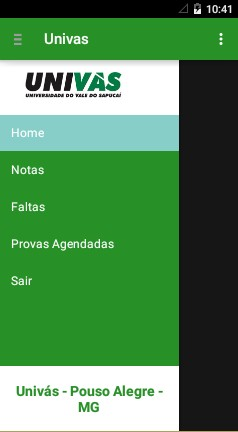
\includegraphics[scale=0.8]{./imagens/3_discussao_resultados/dr.jpg}}
    \caption[Tela principal do aplicativo com as opções de navegação]{Tela
    principal do aplicativo com as opções de navegação.
    \textbf{Fonte:}Elaborado pelos autores.}
    \label{fig:dr}
\end{figure}

    \par Para apresentar as informações, foi utilizado uma lista do tipo
\texttt{ExpandableListView} que segundo \citeonline{android3}, é um
\textit{widget} que exibe uma lista de itens e ao selecionar um desses
elementos, a tela é estendida apresentando os subitens da opção escolhida. Na
Figura \ref{fig:dr1} é mostrada a tela que lista as disciplinas sendo que
Tópicos Avançados está selecionada.


\begin{figure}[h!]
    \centerline{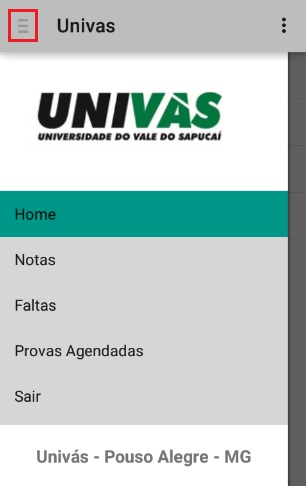
\includegraphics[scale=0.8]{./imagens/3_discussao_resultados/dr1.png}}
    \caption[Lista de disciplinas]{Lista de disciplinas.
        \textbf{Fonte:}Elaborado pelos autores.}
    \label{fig:dr1}
\end{figure}

    \pagebreak

    \par O GCM foi utilizado neste projeto para fazer a transmissão dos eventos do
servidor para o aplicativo. Com ele, a troca de dados tornou-se mais rápido e
simples, pois toda a lógica de entrega fica por conta da Google.

    \par Quando se trata de apenas uma informação para um único dispositivo, o
controle é simples, mas a partir do momento em que há vários equipamentos para
receber informações distintas, o gerenciamento torna-se mais complexo. Por
isso, pode-se afirmar que o GCM solucionou este problema, mostrando-se eficaz
na transmissão dos dados, além de ser de fácil configuração. A Figura
\ref{fig:dr2}, ilustra uma notificação logo após o GCM ter entregue uma
mensagem ao aplicativo. Ao baixar a paleta de notificação será apresentado um
resumo da notificação, como apresenta a Figura \ref{fig:dr3}.


\begin{figure}[h!]
    \centerline{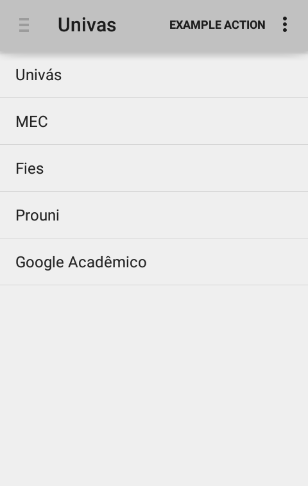
\includegraphics[scale=0.8]{./imagens/3_discussao_resultados/dr2.png}}
    \caption[Notificação na barra de notificações do dispositivo.]{Notificação na
    barra de notificações do dispositivo.
    \textbf{Fonte:}Elaborado pelos autores.}
    \label{fig:dr2}
\end{figure}


\begin{figure}[h!]
    \centerline{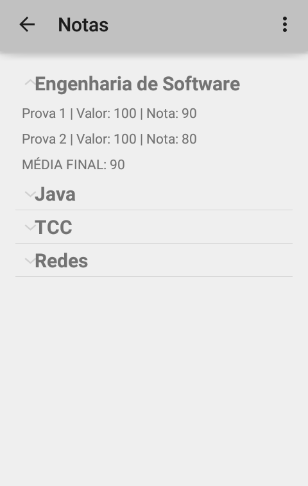
\includegraphics[scale=0.8]{./imagens/3_discussao_resultados/dr3.png}}
    \caption[Paleta de notificação estendida]{Paleta de notificação estendida.
        \textbf{Fonte:}Elaborado pelos autores.}
    \label{fig:dr3}
\end{figure}

\pagebreak

    \par Ao clicar na notificação é apresentado para o aluno a tela que exibe os
dados da notificação. Na Figura \ref{fig:dr4}, pode-se ver a tela exibindo as
informações de um evento de notas.

\begin{figure}[h!]
    \centerline{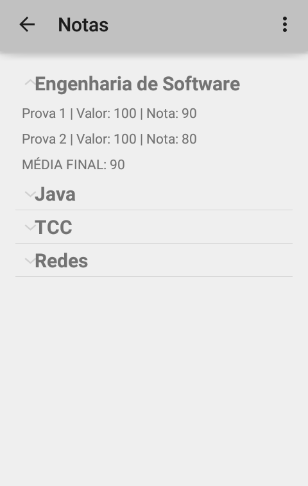
\includegraphics[scale=0.8]{./imagens/3_discussao_resultados/dr4.png}}
    \caption[Tela exibindo os dados após clicado na notificação]{Tela exibindo os
    dados após clicado na notificação.
    \textbf{Fonte:}Elaborado pelos autores.}
    \label{fig:dr4}
\end{figure}

    \par Portanto, sabendo-se que esta pesquisa enquadra-se no tipo de pesquisa
aplicada, o qual tem por finalidade desenvolver um produto real para resolver
um determinado problema e que a solução construída auxilia tanto a Univás, que
terá um nova forma de disponibilizar suas informações, quanto aos alunos, que
possuem a opção de consultarem suas informações acadêmicas através de
dispositivos móveis, entende-se que este trabalho atingiu suas expectativas.    
